\documentclass[conference]{IEEEtran}
% *** CITATION PACKAGES ***
\usepackage[
style=ieee
]{biblatex}
\addbibresource{report.bib} %Imports bibliography file

% *** FLOAT PACKAGES ***
\usepackage{float}

% *** GRAPHICS RELATED PACKAGES ***
\usepackage{graphicx}
\usepackage{caption}
\usepackage{subcaption}

% *** MATH PACKAGES ***
\usepackage{amsmath}

% *** PDF, URL AND HYPERLINK PACKAGES ***
\usepackage{url}

\begin{document}
\title{
  RBE/CS 549 Project 2\\
   Structure from Motion and NeRF \\
  \vspace{0.3cm}
  \large{\textit{Using 2 Late Days}}
}

\author{\IEEEauthorblockN{Blake Bruell}
\IEEEauthorblockA{Worcester Polytechnic Institute\\
babruell@wpi.edu} \and
\IEEEauthorblockN{Cole Parks}
\IEEEauthorblockA{Worcester Polytechnic Institute\\
cparks@wpi.edu}}

\maketitle

\begin{abstract}
This report outlines the process of creating a 3D visualization of a driving scene from a monocular forward facing camera view. The process is broken down into three phases, each of which encompass a certain set of target goals. Techniques were explored and implemented to detect lane lines, detect objects in the scene, localize objects in 3d space, and create a 3D visualization of the scene using Blender. The report also discusses the challenges faced and the results obtained from the implementation of the techniques.
\end{abstract}

\section{Phase 1}
In the first phase of this project our goals were to get basic features of a scene localized in 3D space, including vehicles, lanes, pedestrians, traffic lights, and road signs. To accomplish this, we looked at different possible pipelines for the object detection and localization.

\subsection{Object Detection}
Some techniques for object detection, such as described in \emph{3D Bounding Box Estimation Using Deep Learning and Geometry} \cite{3DBoxEstimation}, will directly output a 3D bounding box of teh detected objects using a single image. These techniques have the distinct advantage of providing all needed information to render the object from a single technique, but in general the performance of these technique can be limited by the fact that are doing so much. In addition, pre-trained weights on classes other than vehicles were not easily available, and as such our team looked for other solutions.

The obvious choice, then was to use a information from multiple different networks, each providing some needed information. At the bare minimum, two networks would be needed: one to detect objects, and one to predict depth. Our team chose solutions which were easy to get running, as we wanted to focus on getting outputs from the networks as quickly as possible. To this end, we elected to use the YoloV9 framework \cite{YOLOv9}, due to its outstanding performance, and also ease of use due to the fantastic Ultralytics framework for YOLO models. The output of the YOLO model is shown in Figure \ref{fig:yolo_output}.

\begin{figure}
    \centering
    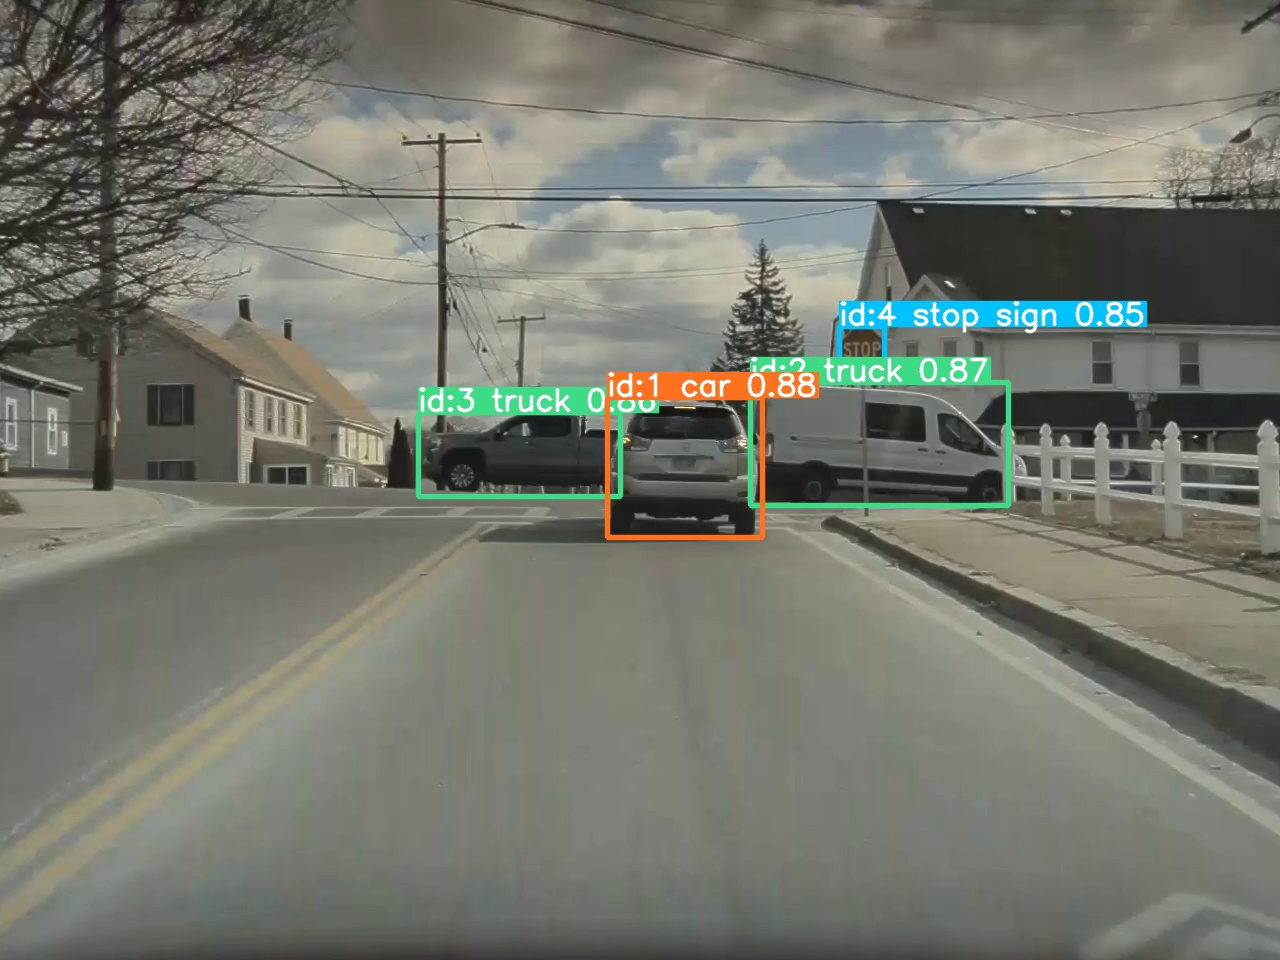
\includegraphics[width=0.95\linewidth]{images/YOLOv9.jpg}
    \caption{Output of YOLO model}
    \label{fig:yolo_output}
\end{figure}

\subsection{Depth Estimation}
For depth estimation, there are many different techniques available. One technique in particular stuck out in the early research that our team did, namely ZoeDepth \cite{ZoeDepth}. ZoeDepth is monocular metric depth estimation technique which builds upon the MiDaS architecture. The ZoeDepth model is trained on both indoor and outdoor scenes, and is able to generalize very well. ZoeDepth also had the distinct advantage of being setup to be run via TorchHub, a online repository of networks. As such, getting the network running, and integrating it into the existing YOLO pipeline was much easier. The output of the ZoeDepth model is shown in Figure \ref{fig:zoe_depth_output}.

\begin{figure}
    \centering
    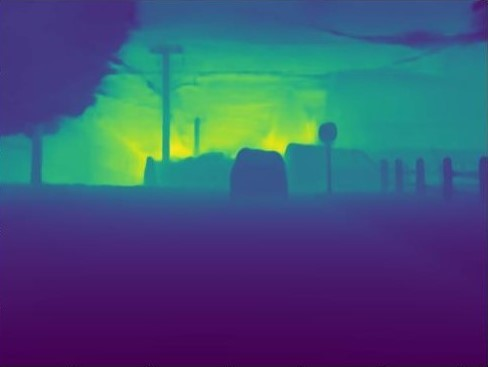
\includegraphics[width=0.95\linewidth]{images/depth.jpg}
    \caption{Output of ZoeDepth model}
    \label{fig:zoe_depth_output}
\end{figure}

\subsection{3D Localization}
Once the outputs from YOLOv9 and ZoeDepth were obtained, the next step was to localize the objects in 3D space. This was done by first taking the center of each bounding box, and then using the depth map to get the depth of the object at the center of the bounding box. The pinhole projection model was then used to get the 3D coordinates of the object.
We began with the pinhole projection model, which is shown in Equation \ref{eq:pinhole_projection}. In this equation, $\lambda$ is a scalar, $\mathbf{K}$ is the camera intrinsics matrix, $\mathbf{R}$ is the rotation matrix, $\mathbf{t}$ is the translation vector, $X$, $Y$, and $Z$ are the 3D coordinates of the object, and $x$ and $y$ are the 2D coordinates of the object in the image.
\begin{equation}\label{eq:pinhole_projection}
    \lambda\begin{bmatrix}
        x \\
        y \\
        1
    \end{bmatrix}
    =
    \mathbf{K}
    \begin{bmatrix}
        \mathbf{R} & \mathbf{t}
    \end{bmatrix}
    \begin{bmatrix}
        X \\
        Y \\
        Z \\
        1
    \end{bmatrix}
\end{equation}
The equation was then simplified by assuming $\mathbf{R}$ and $\mathbf{t}$ are the identity matrix and zero vector, respectively. This simplification is shown in Equation \ref{eq:simplified_pinhole_projection}.
\begin{equation}\label{eq:simplified_pinhole_projection}
    \lambda \mathbf{K}^{-1}\begin{bmatrix}
        x \\
        y \\
        1
    \end{bmatrix}
    =
    \begin{bmatrix}
        X \\
        Y \\
        Z
    \end{bmatrix}
\end{equation}
From this equation, we could get the ray direction of object
\begin{equation}\label{eq:ray_direction}
    \begin{bmatrix}
        X \\
        Y \\
        Z
    \end{bmatrix}
    =
    \lambda \mathbf{K}^{-1}\begin{bmatrix}
        x \\
        y \\
        1
    \end{bmatrix} 
\end{equation}
where $\lambda$ was a normalization factor, so that the magnitude of the ray direction vector was 1. The 3D coordinates of the object were then calculated by multiplying the ray direction vector by the depth of the object at the center of the bounding box, which gave the object's 3D location.

This pipeline was very effective, but it was limited by the fact that the ZoeDepth estimates the depth of the object's surface, and not the center of the object. This meant that the 3D localization was not perfect, but it was still very good. The output of the 3D localization is shown in Figure \ref{fig:3D_localization_output}.

The benefit of this pipeline is that is simple, fast, and applies for all classes of objects that the YOLO model can detect. The downside is that the 3D localization is not perfect, and no information about orientation is provided.

\subsection{3D Rendering}
Finally, to 3D render the scene, a json data-structure was created which contained the 3D coordinates and class of each detected object. This json file was then read in by a Blender python script which placed each object in the scene at the correct location. The output of the 3D rendering is shown in Figure \ref{fig:3D_localization_output}.
\begin{figure}
    \centering
    \begin{subfigure}{0.95\linewidth}
        \centering
        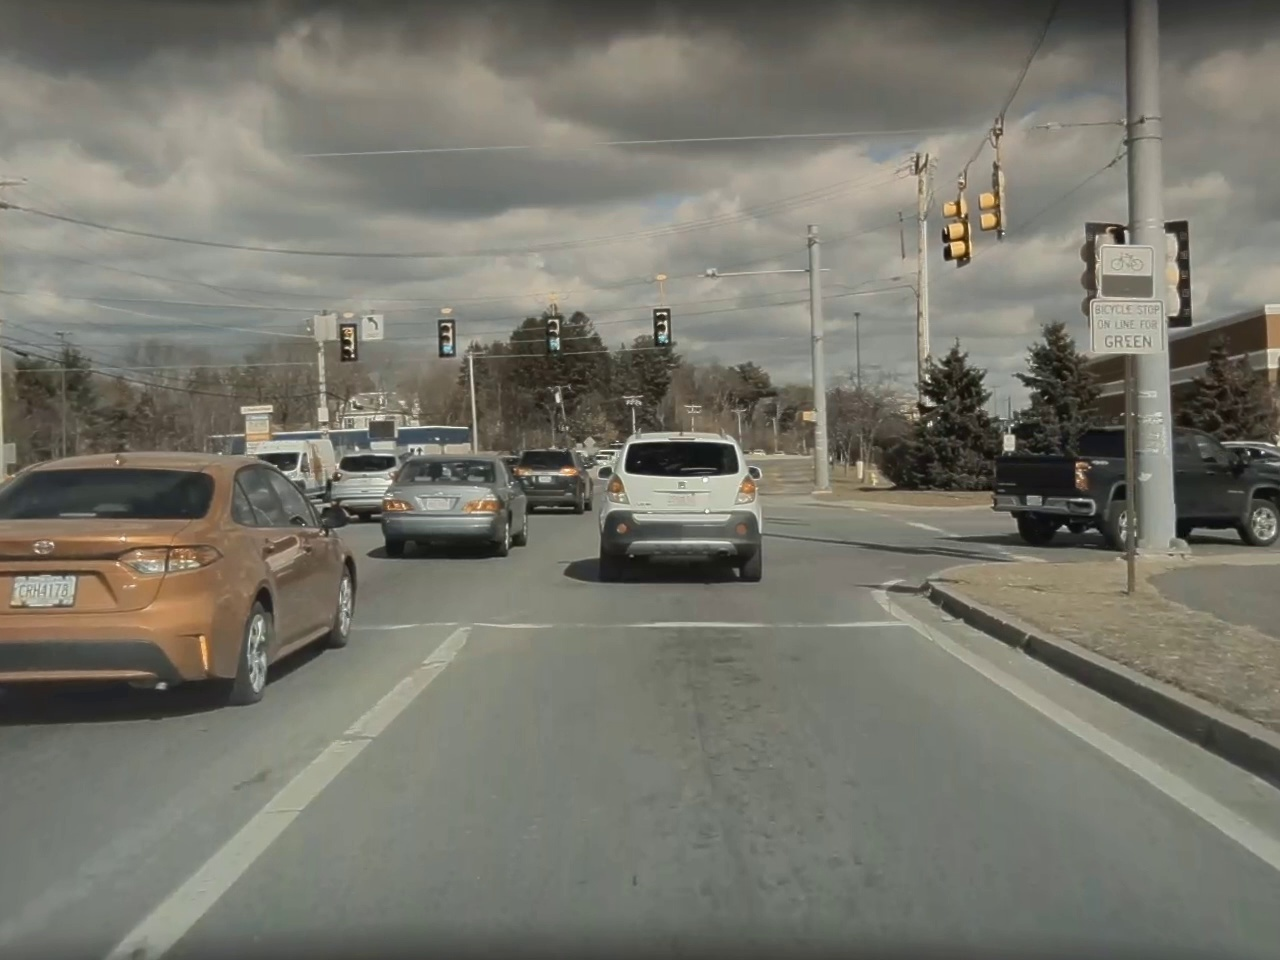
\includegraphics[width=\textwidth]{images/localization_in.jpg}
        \caption{Input image to pipeline.}
    \end{subfigure}
    \begin{subfigure}{0.95\linewidth}
        \centering
        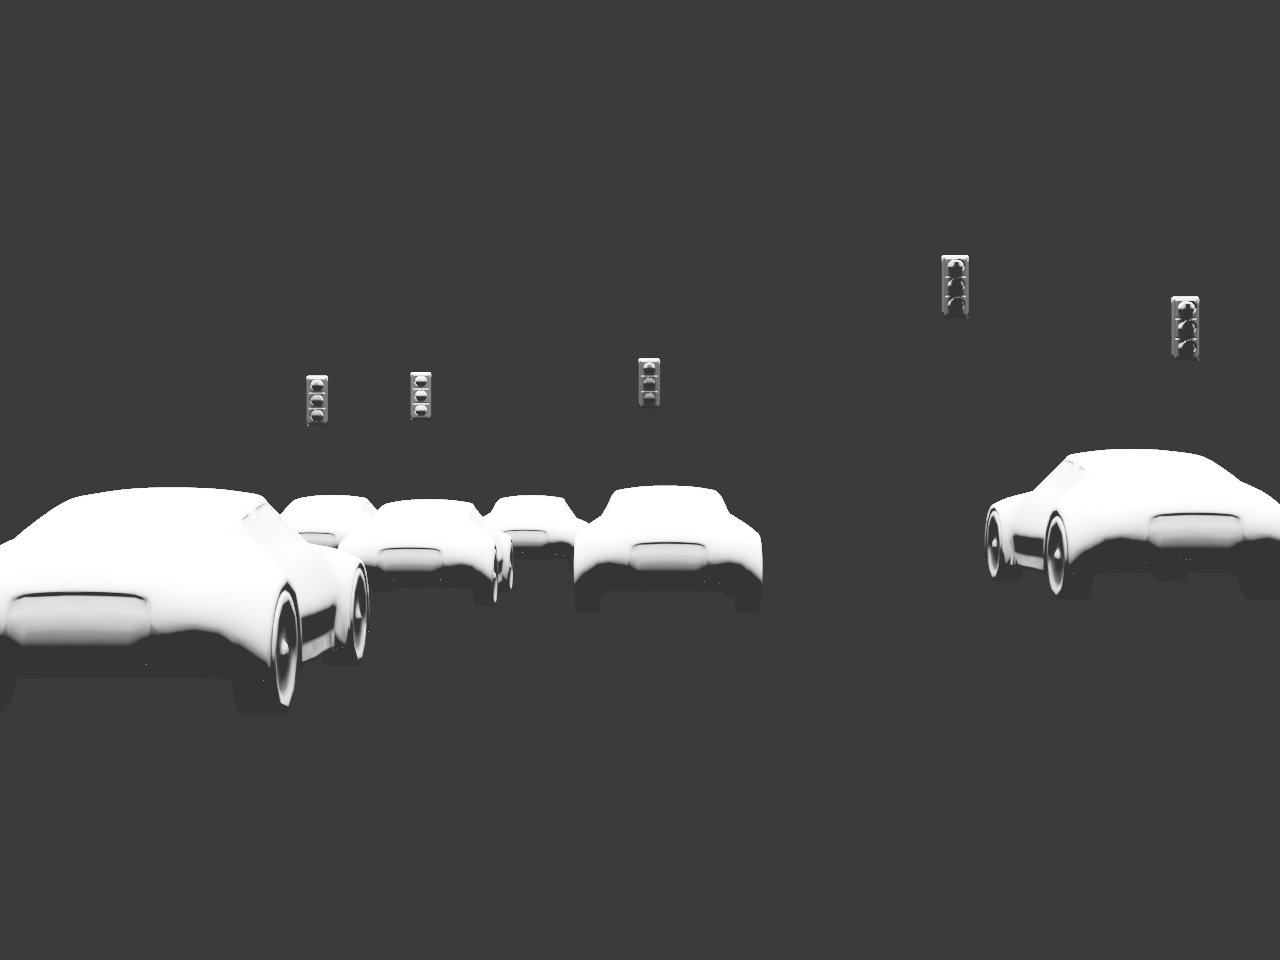
\includegraphics[width=\textwidth]{images/localization.png}
        \caption{Output of 3D localization.}
    \end{subfigure}
    \caption{3D localization of objects.}
    \label{fig:3D_localization_output}
\end{figure}

\subsection{Lane Detection}
There were many choices for lane detection, but we sought to use a technique which gave 3D lane outputs directly. We found many such powerful techniques, such as BEV-LaneDet \cite{BEV-LaneDet} and PersFormer \cite{PersFormer}, but we ran into some serious challenges with getting these networks running. In both cases, the code was publicly available on GitHub, but dependencies were not well documented, and when documented were often many years out of date, making it difficult to setup the environment to run the network. In some cases pre-trained weights were missing, making it difficult to run the test the network, or simply prohibitively expensive to train the network. In many cases, the networks were only setup to be trained and validated on datasets, and not to perform inference on new data. As a result, we were unable to get these networks running in time for the first phase of the project.



\section{Phase 2}

In the second phase of this project, our goals were to successfully detect lanes, traffic light colors and type, and estimate car poses. We began this section by performing a comprehensive literature review to understand the state-of-the-art techniques for each of these tasks. We then moved forward with the techniques which showed the most promise.


\subsection{Lane Detection}
Given that lane detection was missing feature from our Phase 1, we wanted to get this working as soon as possible. The techniques which provided 3D lane output discussed in the previous section were still not working, so our team looked into more techniques. 

\subsubsection{Other 3D Lane Detection Techniques}
Other lane detection techniques were considered, such as Anchor3DLane \cite{Anchor3DLane}. Again, the same issues with functionality were encountered, and proved too time consuming to resolve. As such our team decided to look into techniques which provided lane output in 2D image space.

\subsubsection{Segmentation of Lane Lines}
The first class of technique that we found in the literature were techniques which segmented the lane lines in an image. The first technique we came across was an extension of YOLO for the express purpose of driving perception, called YOLOPv2 \cite{YOLOPv2}. This network not only segmented the lane lines, but also provided segmentation of other regions, such as drivable area, and also detected vehicles in the scene. The output of this paper on our test data is shown in Figure \ref{fig:YOLOPv2_output}. As is apparent in the image, the lane segmentation was not very precise, which would make it difficult to fit 2D lane lines to the output of this network. Even more problematic, the different lane lines were all classified with the same mask. This was a problem, as our rendering pipeline used Bézier curves to interpolate between a set of sampled points of each lane line separately. This meant that the output of this network was not suitable for our purposes.

\begin{figure}
    \centering
    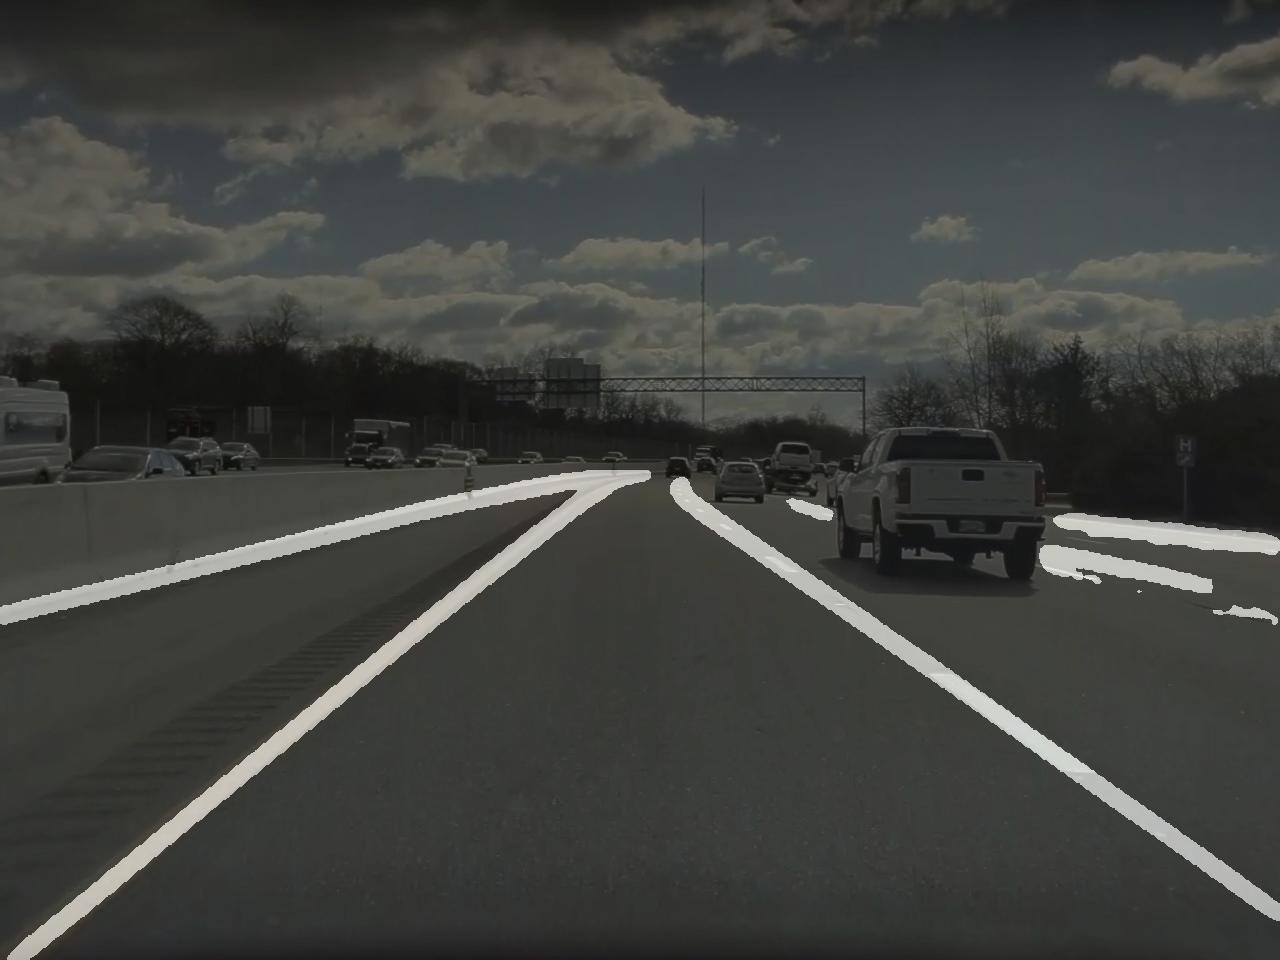
\includegraphics[width=0.9\linewidth]{images/YOLOPv2.jpg}
    \caption{Output of lane detection from YOLOPv2 \cite{YOLOPv2}.}
    \label{fig:YOLOPv2_output}
\end{figure}

Another segmentation technique using a Mask RCNN backbone was considered, but again, the output was not suitable for our pipeline, and the documentation and code for the technique were not as easily available as the YOLOPv2 technique. 


\subsubsection{2D Lane Line Fitting}
The final class of techniques considered would return lane line coordinates fitted to each individual lane line. These techniques were much more useful than the segmentation style 2D detection networks, as we could simply make the assumption that the lanes lay on the ground plane, and project the 2D lane sample points onto the ground plane to recover lane lines. The first technique our team considered was CLRNet \cite{CLRNet}. This network provided decent output, and had documentation on how to run inference with the network on new images. The output of the network is shown in Figure \ref{fig:CLRNet_output}.

Initially, the output of the network was underwhelming, but it was noted that the input images lacked contrast and brightness, and so did not match the training images well. We therefor applied a simple preprocessing step to the images before detecting lanes, which proved effective at improving the output of the network. The output of the network after preprocessing is shown in Figure \ref{fig:CLRNet_output_preprocessed}.

\begin{figure}
    \centering
    \begin{subfigure}{0.95\linewidth}
        \centering
        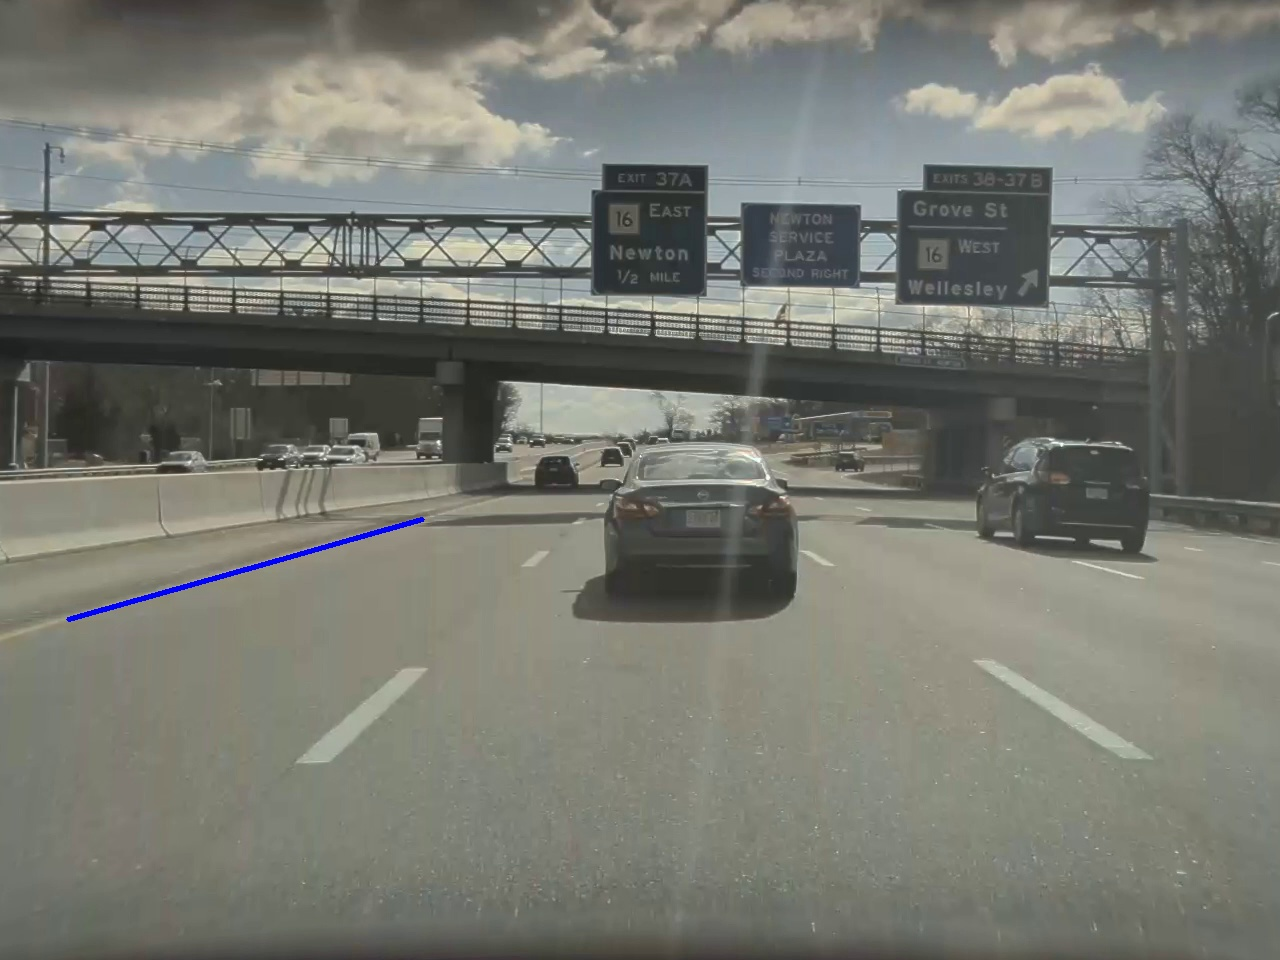
\includegraphics[width=\textwidth]{images/CLRNet_without_proc.jpg}
        \caption{Output of CLRNet before preprocessing.}
        \label{fig:CLRNet_output}
    \end{subfigure}
    \begin{subfigure}{0.95\linewidth}
        \centering
        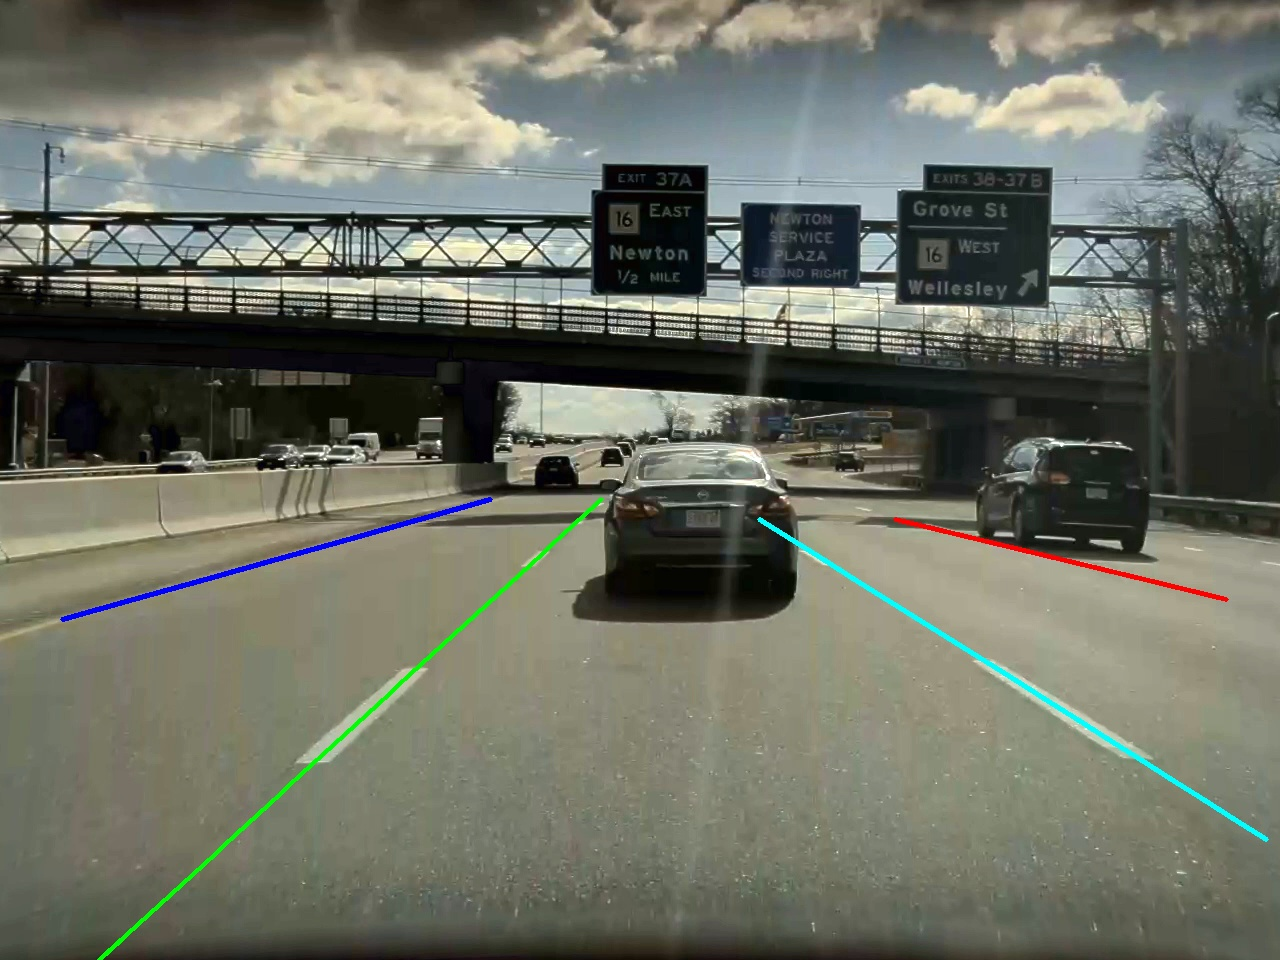
\includegraphics[width=\textwidth]{images/CLRNet_with_proc.jpg}
        \caption{Output of CLRNet after preprocessing.}
        \label{fig:CLRNet_output_preprocessed}
    \end{subfigure}
    \caption{Output of CLRNet \cite{CLRNet}.}
\end{figure}

An extension of CLRNet, discussed in \emph{Recursive Video Lane Detection}, added temporal information to the network greatly improving the consistency of the output on video inputs \cite{RVLD}. Again, the codebase could not be made to function on our test data, and so our team settled on using the CLRNet network for lane detection.

\subsubsection{Lane Line Reprojection}
Once the lane lines were detected, the next step was to re-project the 2D lane lines onto the ground plane. This again began with the pinhole projection model, as described in Equation \ref{eq:pinhole_projection}. We then made the assumption that the camera was looking straight ahead, and that the ground plane was perpendicular to the $XZ$ plane with $Y = -1.5$. This allowed us to simplify the pinhole projection model to the form shown in Equation \ref{eq:simplified_pinhole_projection_2}.
\begin{equation}\label{eq:simplified_pinhole_projection_2}
\begin{aligned}
  \lambda\begin{bmatrix}
    x \\
    y \\
    1
  \end{bmatrix}
  & =
  \mathbf{K}
  \begin{bmatrix}
      \mathbf{I} & \mathbf{0}
  \end{bmatrix}
  \begin{bmatrix}
      X \\
      -1.5 \\
      Z \\
      1
  \end{bmatrix} \\
  \begin{bmatrix}
    X \\
    -1.5 \\
    Z
  \end{bmatrix}
  & =
  \lambda \mathbf{K}^{-1} \begin{bmatrix}
    x \\
    y \\
    1
  \end{bmatrix}
\end{aligned}
\end{equation}
From this equation, we could get the 3D coordinates of the lane lines. The output of the re-projected lane lines is shown in Figure \ref{fig:reprojected_lane_lines}.

\begin{figure}
    \centering
    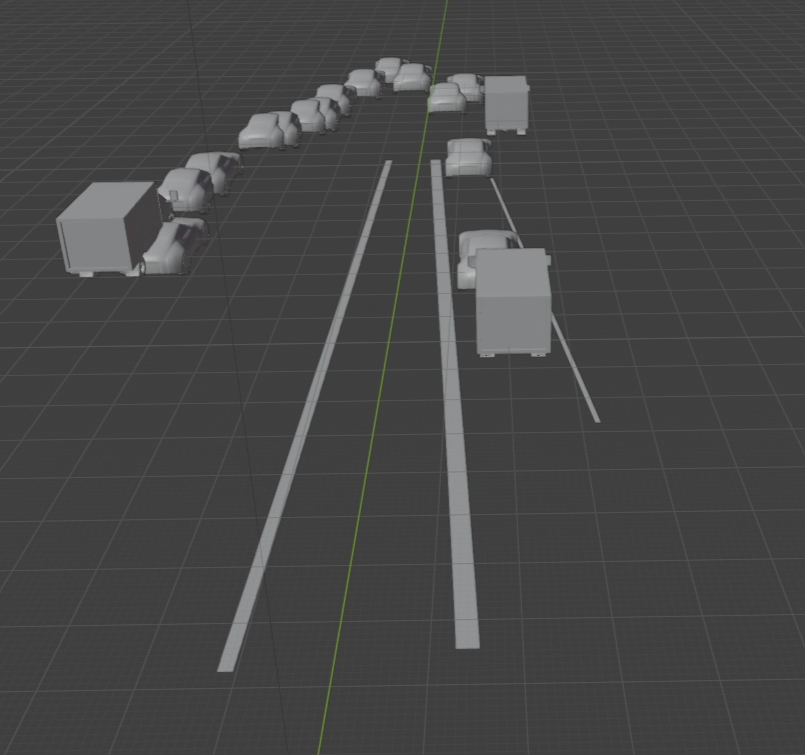
\includegraphics[width=0.95\linewidth]{images/reprojected_lanes.png}
    \caption{Re-projected lane lines.}
    \label{fig:reprojected_lane_lines}
\end{figure}

\subsection{Traffic Light Color Detection}
While the YOLOv9 pipeline from Phase 1 provided 3D localization of traffic lights, it did not provide the color of the traffic light. Our team looked into the literature, and found that some people had fine tuned a YOLO network to detect traffic lights and their colors. We decided to use this technique, as it would fit nicely into our existing pipeline. We used data from cinTA\_v2 dataset to fine tune a YOLOv8 network \cite{CintaV2Dataset}, but the output proved very poor, as detection of traffic lights in the first place was much more inconsistent, and even when detected the color was not correct. Due to time constraints, our team decided to ignore the traffic light color detection for the time being, and focus on the other tasks. 

\subsection{Car Pose Estimation}
Crucially missing from the first phase of this project was the ability to estimate the pose of the cars in the scene. This was a difficult task, as the only information we had about the cars was their bounding boxes. Many techniques have been proposed over the years, but our team turned back to \emph{3D Bounding Box Estimation Using Deep Learning and Geometry} \cite{3DBoxEstimation}, as it not only provided pose of the object, but also the 3D location. The output of the network on data from the dataset the network was trained on is shown in Figure \ref{fig:3DBoxEstimation_output_trained}, and the output of the network on our test data is shown in Figure \ref{fig:3DBoxEstimation_output_test}. As is apparent from the comparison, the network did not generalize well to our test data, or some other issue was present. This failure, along with the fact that networks which predicted both bounding box and pose would preclude the use of the YOLO pipeline, prompted out team to look into other techniques for car pose estimation.

\begin{figure}
    \centering
    \begin{subfigure}{0.95\linewidth}
        \centering
        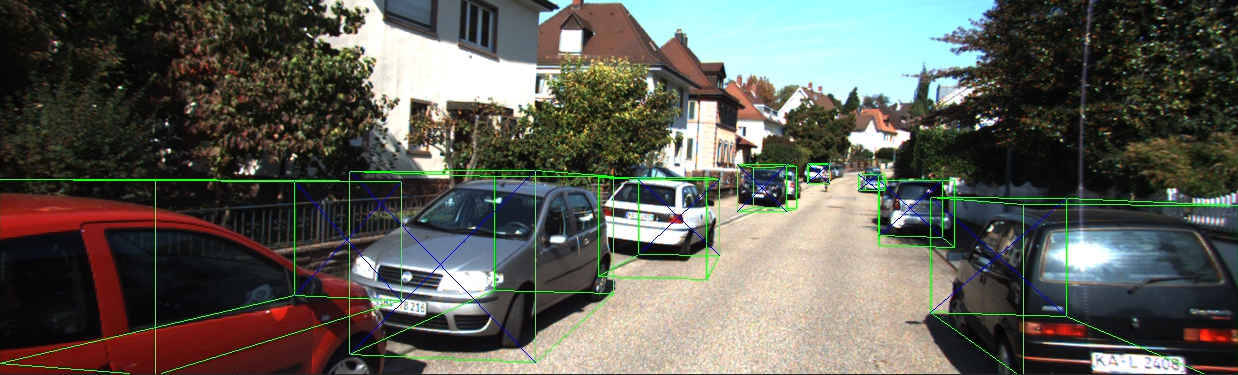
\includegraphics[width=\textwidth]{images/car_pose_train.png}
        \caption{Output on training data.}
        \label{fig:3DBoxEstimation_output_trained}
    \end{subfigure}
    \begin{subfigure}{0.95\linewidth}
        \centering
        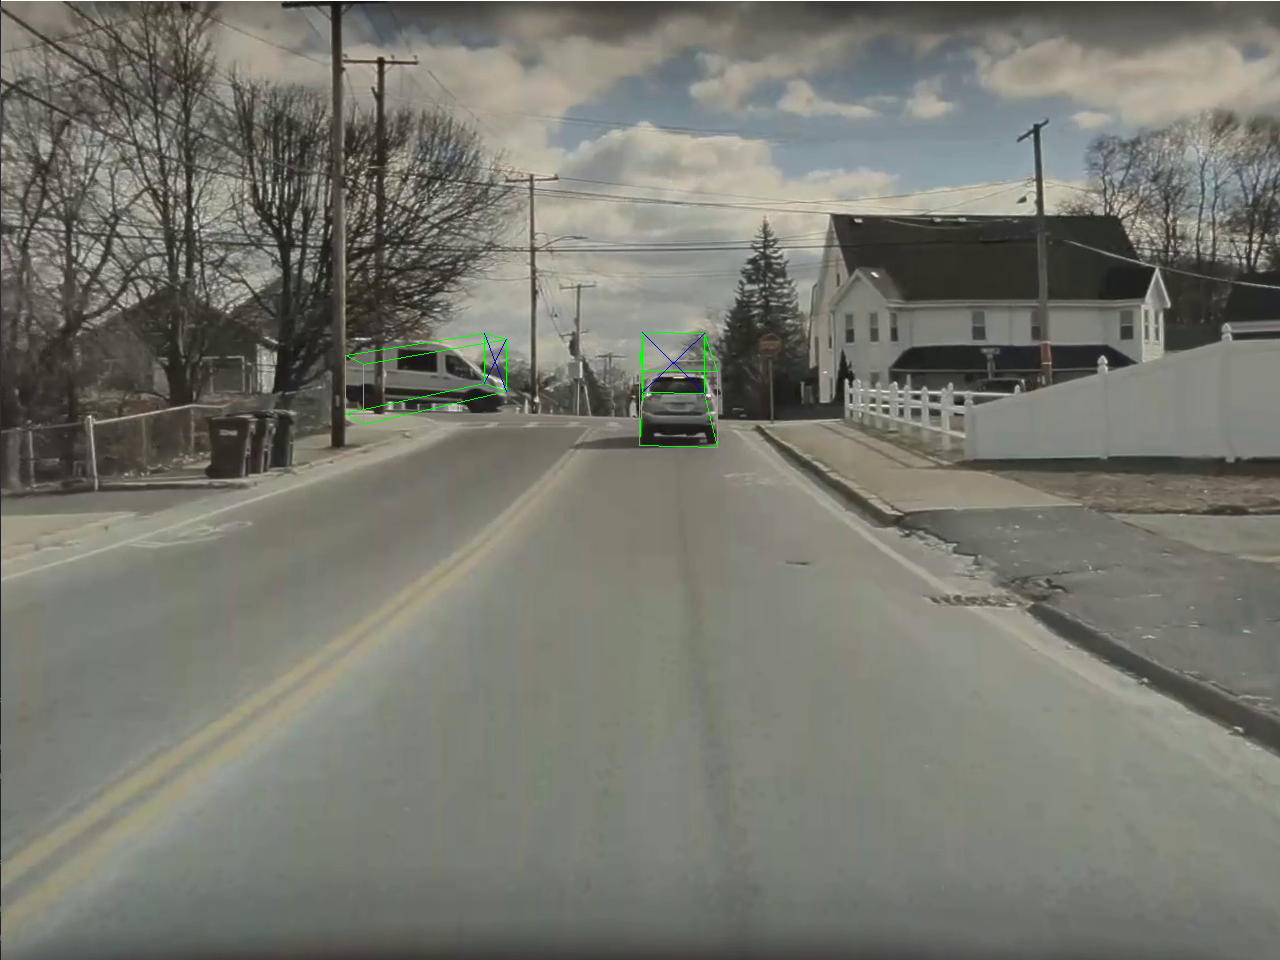
\includegraphics[width=\textwidth]{images/car_pose.png}
        \caption{Output on test data.}
        \label{fig:3DBoxEstimation_output_test}
    \end{subfigure}
    \caption{Output of 3D Bounding Box Estimation Using Deep Learning and Geometry \cite{3DBoxEstimation}.}
\end{figure}

The next technique which our team looked into was called EgoNet \cite{EgoNet}, which had the advantage that it could take in the output of the YOLOv9 network, and then predict the pose of the cars in the scene. The network also came with pre-trained weights, necessary due to our time constraints, but again the code base failed to have good support or documentation on how to run inference on new images. Due to these issues, our team did not include any pose estimation in our pipeline for Phase 2.


\section{Phase 3}
In the third phase of this project, our goals were to flesh out pose detection for cars, and add in the ability to detect traffic light colors, and improve the rendering pipeline so that entire scenes could be rendered in a reasonable amount of time.




\section{Shortcomings}
After completing our entire pipeline, there are clearly some shortcomings, and things our team could simply not get working.

\section{Reflection}

% Our team put in many hours of work into this project, and most of that time was spent attempting to get techniques described in literature to run on our data, or even run at all. We found many powerful techniques, all with source code available, but despite this could not manage to get things actually working in time for the deadlines. This was in part due to time constraints within the group, but also due to the nebulous nature of the project. In previous projects, the goals were very clear, and the techniques could be \emph{fully} understood by our team, and thus knew when we were on the right track or not. With this project in contrast, our team found it hard to judge whether pursuing any given technique was worth our time, and thus found it hard to make progress, as we wanted to avoid committing to a technique which would not work.

% As a result of this, while our team spent considerable time working on this project, it felt like the only way of getting better results was simply dedicating more time to the tedious task of debugging outdated python dependencies. 

% Our team also experienced a lot of fatigue when working on the project, especially in comparison to the previous projects in this course, as we did not feel as though we were learning anything or making progress as we spent dozens of hours struggling to perform inference using techniques we discovered. We didn't feel we had the time implement our own techniques, but also felt as though we were not learning anything by trying to get other people's techniques to work. Since this goal of this project was focused on "good" output, it made it stressful to prioritize different tasks, short of simply putting more time into everything, as there was no guarantee that any given pathway was worthwhile. This was a very frustrating experience for our team. This in turn made it harder to justify taking more than dozens of hours each week we spent on the project, as it felt as though we could have spent many more dozens of hours without making any progress, or learning anything new.

Our team put in many hours of work into this project, and most of that time was spent attempting to get techniques described in literature to run on our data, or even run at all. We found many powerful techniques, all with source code available, but despite this could not manage to get things actually working in time for the deadlines. We noted that the task of reproducing results from pervious papers, and generalizing the code to new data was tedious, and also very exhausting, frustrating, and time consuming. This made it difficult to make progress, as we wanted to avoid committing to a technique which would not work. The unbounded nature of the target goals for this project also made it harder to keep work focused and directed at the most important tasks. To address these challenges, our team frequently created priority lists and split up work into tasks which were entirely parallelizable to ensure that the most worthwhile tasks were completed first, and that work was never held up by the progress of the other individual.

The second aspect of this project which made it difficult to motivate (but something which cannot be avoided with this kind of work) was the fact that the project was not about \emph{understanding} or developing intuition or rigorous knowledge about a topic, but rather was concerned purely with results. This project showed the difficulties with the latter goal, as well as allowed our team to gain a first hand idea of what we enjoyed and did not enjoy about this aspect of the field of computer vision.

On the positive side, while we may not have found the actual work enjoyable, and did not learned much about the actual techniques being used, as it would have simply been too much work, we did learn about the \emph{process} of doing reviews of papers and replicating results. We learned both what makes it challenging and frustrating, and also the value in having experience in doing so. This project gave our team a initial taste of this experience, and also provided a good opportunity to learn about the challenges of working with other people's code, and the importance of good documentation and code quality. The challenges we faced in this project provided motivation to continue to ensure that the code we write is reproducible, understandable, and applicable by others.

\printbibliography
\clearpage
\appendices
\raggedbottom
\section{Results}

\end{document}
